\documentclass[aspectratio=169]{beamer}
% Shared preamble for ml/ slide decks.
% Each lecture .tex starts with:
%   \documentclass[aspectratio=169]{beamer}
%   % Shared preamble for ml/ slide decks.
% Each lecture .tex starts with:
%   \documentclass[aspectratio=169]{beamer}
%   % Shared preamble for ml/ slide decks.
% Each lecture .tex starts with:
%   \documentclass[aspectratio=169]{beamer}
%   \input{../preamble}
% Compile from inside the chapter folder so \input{../preamble} resolves.

\usetheme{default}
\usecolortheme{dove}

\setbeamertemplate{navigation symbols}{}
\setbeamertemplate{footline}{%
  \hfill{\large\insertframenumber\,/\,\inserttotalframenumber}\hspace{0.8em}\vspace{0.5em}%
}

% Project palette (existing, kept for backwards compatibility with deferred/*)
\definecolor{popblue}{RGB}{52, 101, 164}
\definecolor{sampred}{RGB}{204, 0, 0}
\definecolor{paramgreen}{RGB}{0, 140, 70}
\definecolor{warnred}{RGB}{180, 40, 40}
\definecolor{orange1}{RGB}{220, 120, 0}
\definecolor{violet1}{RGB}{120, 50, 160}
\definecolor{lightbg}{RGB}{245, 245, 250}

% Armenian flag palette (use these for any 3-color highlight; per CLAUDE.md).
% "Nice versions": slightly de-saturated from the official spec for slide use,
% so they don't burn out under projector colors. Originals kept as *_pure.
\definecolor{armred}{RGB}{200, 30, 40}      % nice red (official #D90012 muted)
\definecolor{armblue}{RGB}{30, 70, 160}     % nice blue (official #0033A0 muted)
\definecolor{armorange}{RGB}{230, 160, 30}  % nice orange (official #F2A800 muted)
\definecolor{armred_pure}{HTML}{D90012}     % official Armenian flag red
\definecolor{armblue_pure}{HTML}{0033A0}    % official Armenian flag blue
\definecolor{armorange_pure}{HTML}{F2A800}  % official Armenian flag orange

\setbeamercolor{frametitle}{fg=popblue}
\setbeamercolor{title}{fg=popblue}

\usepackage{pgfplots}
\usepackage{tikz}
\usetikzlibrary{shapes, arrows.meta, positioning, calc, decorations.pathreplacing, patterns, matrix}
\pgfplotsset{compat=1.18}
\usepackage{amsmath, amssymb, amsfonts}
\usepackage{bm}
\usepackage{dsfont}
\usepackage{array}
\usepackage{pifont}
\usepackage{colortbl}
\usepackage{fontenc}

% Callout boxes. Purely additive - existing decks are unaffected.
% Usage: \begin{tcolorbox}[colback=armblue!8, colframe=armblue, boxrule=0.6pt, arc=2pt,
%                          title=\textbf{Key idea}] ... \end{tcolorbox}
% Palette convention (ml/SLIDE_STYLE.md): armblue=key idea, armred=trap/warning,
% paramgreen=takeaway or "Next", armorange=watch-out.
\usepackage[most]{tcolorbox}

% Cleaner table rules (\toprule, \midrule, \bottomrule). Also purely additive.
\usepackage{booktabs}

% \cancel{...} for struck-through terms in derivations (added 2026-08-11 for the
% importance-sampling frame in ch11_rl, where the dynamics cancel). Purely additive.
\usepackage{cancel}

% Minimal ML notation macros (subset of slds-lmu latex-math/basic-ml.tex).
% Kept here so we don't have to inline-expand every \thetav, \xv, etc.
% when porting upstream slides.
\newcommand{\R}{\mathds{R}}
\newcommand{\N}{\mathds{N}}
\newcommand{\E}{\mathds{E}}
\newcommand{\Xspace}{\mathcal{X}}
\newcommand{\Yspace}{\mathcal{Y}}
\newcommand{\Hspace}{\mathcal{H}}
\newcommand{\D}{\mathcal{D}}
\newcommand{\Dtrain}{\mathcal{D}_{\text{train}}}
\newcommand{\Dtest}{\mathcal{D}_{\text{test}}}
\newcommand{\xv}{\mathbf{x}}
\newcommand{\yv}{\mathbf{y}}
\newcommand{\Xmat}{\mathbf{X}}
\newcommand{\id}{\mathbf{I}}
\newcommand{\thetav}{\bm{\theta}}
\newcommand{\thetah}{\hat{\bm{\theta}}}
\newcommand{\lamv}{\bm{\lambda}}
\newcommand{\fx}{f(\xv)}
\newcommand{\fxt}{f(\xv \,|\, \bm{\theta})}
\newcommand{\fxi}{f\!\left(\xv^{(i)}\right)}
\newcommand{\fh}{\hat{f}}
\newcommand{\fxh}{\hat{f}(\xv)}
\newcommand{\yh}{\hat{y}}
\newcommand{\yih}{\hat{y}^{(i)}}
% \xi clashes with the Greek letter \xi; write \xv^{(i)} inline instead.
\newcommand{\yi}[1][i]{y^{(#1)}}
\newcommand{\xyi}[1][i]{\left(\xv^{(#1)},\, y^{(#1)}\right)}
\newcommand{\thx}{\bm{\theta}^\top \xv}
\newcommand{\sumin}{\sum_{i=1}^{n}}
\newcommand{\sumjp}{\sum_{j=1}^{p}}
\newcommand{\Lxy}{L\!\left(y, \fx\right)}
\newcommand{\Lxyi}{L\!\left(\yi, \fxi\right)}
\newcommand{\risk}{\mathcal{R}}
\newcommand{\riske}{\mathcal{R}_{\text{emp}}}
\newcommand{\risket}{\mathcal{R}_{\text{emp}}(\bm{\theta})}
\newcommand{\riskt}{\mathcal{R}(\bm{\theta})}
\newcommand{\riskr}{\mathcal{R}_{\text{reg}}}
\newcommand{\argmin}{\mathop{\mathrm{arg\,min}}}
\newcommand{\argmax}{\mathop{\mathrm{arg\,max}}}
\newcommand{\eps}{\varepsilon}

% Compile from inside the chapter folder so % Shared preamble for ml/ slide decks.
% Each lecture .tex starts with:
%   \documentclass[aspectratio=169]{beamer}
%   \input{../preamble}
% Compile from inside the chapter folder so \input{../preamble} resolves.

\usetheme{default}
\usecolortheme{dove}

\setbeamertemplate{navigation symbols}{}
\setbeamertemplate{footline}{%
  \hfill{\large\insertframenumber\,/\,\inserttotalframenumber}\hspace{0.8em}\vspace{0.5em}%
}

% Project palette (existing, kept for backwards compatibility with deferred/*)
\definecolor{popblue}{RGB}{52, 101, 164}
\definecolor{sampred}{RGB}{204, 0, 0}
\definecolor{paramgreen}{RGB}{0, 140, 70}
\definecolor{warnred}{RGB}{180, 40, 40}
\definecolor{orange1}{RGB}{220, 120, 0}
\definecolor{violet1}{RGB}{120, 50, 160}
\definecolor{lightbg}{RGB}{245, 245, 250}

% Armenian flag palette (use these for any 3-color highlight; per CLAUDE.md).
% "Nice versions": slightly de-saturated from the official spec for slide use,
% so they don't burn out under projector colors. Originals kept as *_pure.
\definecolor{armred}{RGB}{200, 30, 40}      % nice red (official #D90012 muted)
\definecolor{armblue}{RGB}{30, 70, 160}     % nice blue (official #0033A0 muted)
\definecolor{armorange}{RGB}{230, 160, 30}  % nice orange (official #F2A800 muted)
\definecolor{armred_pure}{HTML}{D90012}     % official Armenian flag red
\definecolor{armblue_pure}{HTML}{0033A0}    % official Armenian flag blue
\definecolor{armorange_pure}{HTML}{F2A800}  % official Armenian flag orange

\setbeamercolor{frametitle}{fg=popblue}
\setbeamercolor{title}{fg=popblue}

\usepackage{pgfplots}
\usepackage{tikz}
\usetikzlibrary{shapes, arrows.meta, positioning, calc, decorations.pathreplacing, patterns, matrix}
\pgfplotsset{compat=1.18}
\usepackage{amsmath, amssymb, amsfonts}
\usepackage{bm}
\usepackage{dsfont}
\usepackage{array}
\usepackage{pifont}
\usepackage{colortbl}
\usepackage{fontenc}

% Callout boxes. Purely additive - existing decks are unaffected.
% Usage: \begin{tcolorbox}[colback=armblue!8, colframe=armblue, boxrule=0.6pt, arc=2pt,
%                          title=\textbf{Key idea}] ... \end{tcolorbox}
% Palette convention (ml/SLIDE_STYLE.md): armblue=key idea, armred=trap/warning,
% paramgreen=takeaway or "Next", armorange=watch-out.
\usepackage[most]{tcolorbox}

% Cleaner table rules (\toprule, \midrule, \bottomrule). Also purely additive.
\usepackage{booktabs}

% \cancel{...} for struck-through terms in derivations (added 2026-08-11 for the
% importance-sampling frame in ch11_rl, where the dynamics cancel). Purely additive.
\usepackage{cancel}

% Minimal ML notation macros (subset of slds-lmu latex-math/basic-ml.tex).
% Kept here so we don't have to inline-expand every \thetav, \xv, etc.
% when porting upstream slides.
\newcommand{\R}{\mathds{R}}
\newcommand{\N}{\mathds{N}}
\newcommand{\E}{\mathds{E}}
\newcommand{\Xspace}{\mathcal{X}}
\newcommand{\Yspace}{\mathcal{Y}}
\newcommand{\Hspace}{\mathcal{H}}
\newcommand{\D}{\mathcal{D}}
\newcommand{\Dtrain}{\mathcal{D}_{\text{train}}}
\newcommand{\Dtest}{\mathcal{D}_{\text{test}}}
\newcommand{\xv}{\mathbf{x}}
\newcommand{\yv}{\mathbf{y}}
\newcommand{\Xmat}{\mathbf{X}}
\newcommand{\id}{\mathbf{I}}
\newcommand{\thetav}{\bm{\theta}}
\newcommand{\thetah}{\hat{\bm{\theta}}}
\newcommand{\lamv}{\bm{\lambda}}
\newcommand{\fx}{f(\xv)}
\newcommand{\fxt}{f(\xv \,|\, \bm{\theta})}
\newcommand{\fxi}{f\!\left(\xv^{(i)}\right)}
\newcommand{\fh}{\hat{f}}
\newcommand{\fxh}{\hat{f}(\xv)}
\newcommand{\yh}{\hat{y}}
\newcommand{\yih}{\hat{y}^{(i)}}
% \xi clashes with the Greek letter \xi; write \xv^{(i)} inline instead.
\newcommand{\yi}[1][i]{y^{(#1)}}
\newcommand{\xyi}[1][i]{\left(\xv^{(#1)},\, y^{(#1)}\right)}
\newcommand{\thx}{\bm{\theta}^\top \xv}
\newcommand{\sumin}{\sum_{i=1}^{n}}
\newcommand{\sumjp}{\sum_{j=1}^{p}}
\newcommand{\Lxy}{L\!\left(y, \fx\right)}
\newcommand{\Lxyi}{L\!\left(\yi, \fxi\right)}
\newcommand{\risk}{\mathcal{R}}
\newcommand{\riske}{\mathcal{R}_{\text{emp}}}
\newcommand{\risket}{\mathcal{R}_{\text{emp}}(\bm{\theta})}
\newcommand{\riskt}{\mathcal{R}(\bm{\theta})}
\newcommand{\riskr}{\mathcal{R}_{\text{reg}}}
\newcommand{\argmin}{\mathop{\mathrm{arg\,min}}}
\newcommand{\argmax}{\mathop{\mathrm{arg\,max}}}
\newcommand{\eps}{\varepsilon}
 resolves.

\usetheme{default}
\usecolortheme{dove}

\setbeamertemplate{navigation symbols}{}
\setbeamertemplate{footline}{%
  \hfill{\large\insertframenumber\,/\,\inserttotalframenumber}\hspace{0.8em}\vspace{0.5em}%
}

% Project palette (existing, kept for backwards compatibility with deferred/*)
\definecolor{popblue}{RGB}{52, 101, 164}
\definecolor{sampred}{RGB}{204, 0, 0}
\definecolor{paramgreen}{RGB}{0, 140, 70}
\definecolor{warnred}{RGB}{180, 40, 40}
\definecolor{orange1}{RGB}{220, 120, 0}
\definecolor{violet1}{RGB}{120, 50, 160}
\definecolor{lightbg}{RGB}{245, 245, 250}

% Armenian flag palette (use these for any 3-color highlight; per CLAUDE.md).
% "Nice versions": slightly de-saturated from the official spec for slide use,
% so they don't burn out under projector colors. Originals kept as *_pure.
\definecolor{armred}{RGB}{200, 30, 40}      % nice red (official #D90012 muted)
\definecolor{armblue}{RGB}{30, 70, 160}     % nice blue (official #0033A0 muted)
\definecolor{armorange}{RGB}{230, 160, 30}  % nice orange (official #F2A800 muted)
\definecolor{armred_pure}{HTML}{D90012}     % official Armenian flag red
\definecolor{armblue_pure}{HTML}{0033A0}    % official Armenian flag blue
\definecolor{armorange_pure}{HTML}{F2A800}  % official Armenian flag orange

\setbeamercolor{frametitle}{fg=popblue}
\setbeamercolor{title}{fg=popblue}

\usepackage{pgfplots}
\usepackage{tikz}
\usetikzlibrary{shapes, arrows.meta, positioning, calc, decorations.pathreplacing, patterns, matrix}
\pgfplotsset{compat=1.18}
\usepackage{amsmath, amssymb, amsfonts}
\usepackage{bm}
\usepackage{dsfont}
\usepackage{array}
\usepackage{pifont}
\usepackage{colortbl}
\usepackage{fontenc}

% Callout boxes. Purely additive - existing decks are unaffected.
% Usage: \begin{tcolorbox}[colback=armblue!8, colframe=armblue, boxrule=0.6pt, arc=2pt,
%                          title=\textbf{Key idea}] ... \end{tcolorbox}
% Palette convention (ml/SLIDE_STYLE.md): armblue=key idea, armred=trap/warning,
% paramgreen=takeaway or "Next", armorange=watch-out.
\usepackage[most]{tcolorbox}

% Cleaner table rules (\toprule, \midrule, \bottomrule). Also purely additive.
\usepackage{booktabs}

% \cancel{...} for struck-through terms in derivations (added 2026-08-11 for the
% importance-sampling frame in ch11_rl, where the dynamics cancel). Purely additive.
\usepackage{cancel}

% Minimal ML notation macros (subset of slds-lmu latex-math/basic-ml.tex).
% Kept here so we don't have to inline-expand every \thetav, \xv, etc.
% when porting upstream slides.
\newcommand{\R}{\mathds{R}}
\newcommand{\N}{\mathds{N}}
\newcommand{\E}{\mathds{E}}
\newcommand{\Xspace}{\mathcal{X}}
\newcommand{\Yspace}{\mathcal{Y}}
\newcommand{\Hspace}{\mathcal{H}}
\newcommand{\D}{\mathcal{D}}
\newcommand{\Dtrain}{\mathcal{D}_{\text{train}}}
\newcommand{\Dtest}{\mathcal{D}_{\text{test}}}
\newcommand{\xv}{\mathbf{x}}
\newcommand{\yv}{\mathbf{y}}
\newcommand{\Xmat}{\mathbf{X}}
\newcommand{\id}{\mathbf{I}}
\newcommand{\thetav}{\bm{\theta}}
\newcommand{\thetah}{\hat{\bm{\theta}}}
\newcommand{\lamv}{\bm{\lambda}}
\newcommand{\fx}{f(\xv)}
\newcommand{\fxt}{f(\xv \,|\, \bm{\theta})}
\newcommand{\fxi}{f\!\left(\xv^{(i)}\right)}
\newcommand{\fh}{\hat{f}}
\newcommand{\fxh}{\hat{f}(\xv)}
\newcommand{\yh}{\hat{y}}
\newcommand{\yih}{\hat{y}^{(i)}}
% \xi clashes with the Greek letter \xi; write \xv^{(i)} inline instead.
\newcommand{\yi}[1][i]{y^{(#1)}}
\newcommand{\xyi}[1][i]{\left(\xv^{(#1)},\, y^{(#1)}\right)}
\newcommand{\thx}{\bm{\theta}^\top \xv}
\newcommand{\sumin}{\sum_{i=1}^{n}}
\newcommand{\sumjp}{\sum_{j=1}^{p}}
\newcommand{\Lxy}{L\!\left(y, \fx\right)}
\newcommand{\Lxyi}{L\!\left(\yi, \fxi\right)}
\newcommand{\risk}{\mathcal{R}}
\newcommand{\riske}{\mathcal{R}_{\text{emp}}}
\newcommand{\risket}{\mathcal{R}_{\text{emp}}(\bm{\theta})}
\newcommand{\riskt}{\mathcal{R}(\bm{\theta})}
\newcommand{\riskr}{\mathcal{R}_{\text{reg}}}
\newcommand{\argmin}{\mathop{\mathrm{arg\,min}}}
\newcommand{\argmax}{\mathop{\mathrm{arg\,max}}}
\newcommand{\eps}{\varepsilon}

% Compile from inside the chapter folder so % Shared preamble for ml/ slide decks.
% Each lecture .tex starts with:
%   \documentclass[aspectratio=169]{beamer}
%   % Shared preamble for ml/ slide decks.
% Each lecture .tex starts with:
%   \documentclass[aspectratio=169]{beamer}
%   \input{../preamble}
% Compile from inside the chapter folder so \input{../preamble} resolves.

\usetheme{default}
\usecolortheme{dove}

\setbeamertemplate{navigation symbols}{}
\setbeamertemplate{footline}{%
  \hfill{\large\insertframenumber\,/\,\inserttotalframenumber}\hspace{0.8em}\vspace{0.5em}%
}

% Project palette (existing, kept for backwards compatibility with deferred/*)
\definecolor{popblue}{RGB}{52, 101, 164}
\definecolor{sampred}{RGB}{204, 0, 0}
\definecolor{paramgreen}{RGB}{0, 140, 70}
\definecolor{warnred}{RGB}{180, 40, 40}
\definecolor{orange1}{RGB}{220, 120, 0}
\definecolor{violet1}{RGB}{120, 50, 160}
\definecolor{lightbg}{RGB}{245, 245, 250}

% Armenian flag palette (use these for any 3-color highlight; per CLAUDE.md).
% "Nice versions": slightly de-saturated from the official spec for slide use,
% so they don't burn out under projector colors. Originals kept as *_pure.
\definecolor{armred}{RGB}{200, 30, 40}      % nice red (official #D90012 muted)
\definecolor{armblue}{RGB}{30, 70, 160}     % nice blue (official #0033A0 muted)
\definecolor{armorange}{RGB}{230, 160, 30}  % nice orange (official #F2A800 muted)
\definecolor{armred_pure}{HTML}{D90012}     % official Armenian flag red
\definecolor{armblue_pure}{HTML}{0033A0}    % official Armenian flag blue
\definecolor{armorange_pure}{HTML}{F2A800}  % official Armenian flag orange

\setbeamercolor{frametitle}{fg=popblue}
\setbeamercolor{title}{fg=popblue}

\usepackage{pgfplots}
\usepackage{tikz}
\usetikzlibrary{shapes, arrows.meta, positioning, calc, decorations.pathreplacing, patterns, matrix}
\pgfplotsset{compat=1.18}
\usepackage{amsmath, amssymb, amsfonts}
\usepackage{bm}
\usepackage{dsfont}
\usepackage{array}
\usepackage{pifont}
\usepackage{colortbl}
\usepackage{fontenc}

% Callout boxes. Purely additive - existing decks are unaffected.
% Usage: \begin{tcolorbox}[colback=armblue!8, colframe=armblue, boxrule=0.6pt, arc=2pt,
%                          title=\textbf{Key idea}] ... \end{tcolorbox}
% Palette convention (ml/SLIDE_STYLE.md): armblue=key idea, armred=trap/warning,
% paramgreen=takeaway or "Next", armorange=watch-out.
\usepackage[most]{tcolorbox}

% Cleaner table rules (\toprule, \midrule, \bottomrule). Also purely additive.
\usepackage{booktabs}

% \cancel{...} for struck-through terms in derivations (added 2026-08-11 for the
% importance-sampling frame in ch11_rl, where the dynamics cancel). Purely additive.
\usepackage{cancel}

% Minimal ML notation macros (subset of slds-lmu latex-math/basic-ml.tex).
% Kept here so we don't have to inline-expand every \thetav, \xv, etc.
% when porting upstream slides.
\newcommand{\R}{\mathds{R}}
\newcommand{\N}{\mathds{N}}
\newcommand{\E}{\mathds{E}}
\newcommand{\Xspace}{\mathcal{X}}
\newcommand{\Yspace}{\mathcal{Y}}
\newcommand{\Hspace}{\mathcal{H}}
\newcommand{\D}{\mathcal{D}}
\newcommand{\Dtrain}{\mathcal{D}_{\text{train}}}
\newcommand{\Dtest}{\mathcal{D}_{\text{test}}}
\newcommand{\xv}{\mathbf{x}}
\newcommand{\yv}{\mathbf{y}}
\newcommand{\Xmat}{\mathbf{X}}
\newcommand{\id}{\mathbf{I}}
\newcommand{\thetav}{\bm{\theta}}
\newcommand{\thetah}{\hat{\bm{\theta}}}
\newcommand{\lamv}{\bm{\lambda}}
\newcommand{\fx}{f(\xv)}
\newcommand{\fxt}{f(\xv \,|\, \bm{\theta})}
\newcommand{\fxi}{f\!\left(\xv^{(i)}\right)}
\newcommand{\fh}{\hat{f}}
\newcommand{\fxh}{\hat{f}(\xv)}
\newcommand{\yh}{\hat{y}}
\newcommand{\yih}{\hat{y}^{(i)}}
% \xi clashes with the Greek letter \xi; write \xv^{(i)} inline instead.
\newcommand{\yi}[1][i]{y^{(#1)}}
\newcommand{\xyi}[1][i]{\left(\xv^{(#1)},\, y^{(#1)}\right)}
\newcommand{\thx}{\bm{\theta}^\top \xv}
\newcommand{\sumin}{\sum_{i=1}^{n}}
\newcommand{\sumjp}{\sum_{j=1}^{p}}
\newcommand{\Lxy}{L\!\left(y, \fx\right)}
\newcommand{\Lxyi}{L\!\left(\yi, \fxi\right)}
\newcommand{\risk}{\mathcal{R}}
\newcommand{\riske}{\mathcal{R}_{\text{emp}}}
\newcommand{\risket}{\mathcal{R}_{\text{emp}}(\bm{\theta})}
\newcommand{\riskt}{\mathcal{R}(\bm{\theta})}
\newcommand{\riskr}{\mathcal{R}_{\text{reg}}}
\newcommand{\argmin}{\mathop{\mathrm{arg\,min}}}
\newcommand{\argmax}{\mathop{\mathrm{arg\,max}}}
\newcommand{\eps}{\varepsilon}

% Compile from inside the chapter folder so % Shared preamble for ml/ slide decks.
% Each lecture .tex starts with:
%   \documentclass[aspectratio=169]{beamer}
%   \input{../preamble}
% Compile from inside the chapter folder so \input{../preamble} resolves.

\usetheme{default}
\usecolortheme{dove}

\setbeamertemplate{navigation symbols}{}
\setbeamertemplate{footline}{%
  \hfill{\large\insertframenumber\,/\,\inserttotalframenumber}\hspace{0.8em}\vspace{0.5em}%
}

% Project palette (existing, kept for backwards compatibility with deferred/*)
\definecolor{popblue}{RGB}{52, 101, 164}
\definecolor{sampred}{RGB}{204, 0, 0}
\definecolor{paramgreen}{RGB}{0, 140, 70}
\definecolor{warnred}{RGB}{180, 40, 40}
\definecolor{orange1}{RGB}{220, 120, 0}
\definecolor{violet1}{RGB}{120, 50, 160}
\definecolor{lightbg}{RGB}{245, 245, 250}

% Armenian flag palette (use these for any 3-color highlight; per CLAUDE.md).
% "Nice versions": slightly de-saturated from the official spec for slide use,
% so they don't burn out under projector colors. Originals kept as *_pure.
\definecolor{armred}{RGB}{200, 30, 40}      % nice red (official #D90012 muted)
\definecolor{armblue}{RGB}{30, 70, 160}     % nice blue (official #0033A0 muted)
\definecolor{armorange}{RGB}{230, 160, 30}  % nice orange (official #F2A800 muted)
\definecolor{armred_pure}{HTML}{D90012}     % official Armenian flag red
\definecolor{armblue_pure}{HTML}{0033A0}    % official Armenian flag blue
\definecolor{armorange_pure}{HTML}{F2A800}  % official Armenian flag orange

\setbeamercolor{frametitle}{fg=popblue}
\setbeamercolor{title}{fg=popblue}

\usepackage{pgfplots}
\usepackage{tikz}
\usetikzlibrary{shapes, arrows.meta, positioning, calc, decorations.pathreplacing, patterns, matrix}
\pgfplotsset{compat=1.18}
\usepackage{amsmath, amssymb, amsfonts}
\usepackage{bm}
\usepackage{dsfont}
\usepackage{array}
\usepackage{pifont}
\usepackage{colortbl}
\usepackage{fontenc}

% Callout boxes. Purely additive - existing decks are unaffected.
% Usage: \begin{tcolorbox}[colback=armblue!8, colframe=armblue, boxrule=0.6pt, arc=2pt,
%                          title=\textbf{Key idea}] ... \end{tcolorbox}
% Palette convention (ml/SLIDE_STYLE.md): armblue=key idea, armred=trap/warning,
% paramgreen=takeaway or "Next", armorange=watch-out.
\usepackage[most]{tcolorbox}

% Cleaner table rules (\toprule, \midrule, \bottomrule). Also purely additive.
\usepackage{booktabs}

% \cancel{...} for struck-through terms in derivations (added 2026-08-11 for the
% importance-sampling frame in ch11_rl, where the dynamics cancel). Purely additive.
\usepackage{cancel}

% Minimal ML notation macros (subset of slds-lmu latex-math/basic-ml.tex).
% Kept here so we don't have to inline-expand every \thetav, \xv, etc.
% when porting upstream slides.
\newcommand{\R}{\mathds{R}}
\newcommand{\N}{\mathds{N}}
\newcommand{\E}{\mathds{E}}
\newcommand{\Xspace}{\mathcal{X}}
\newcommand{\Yspace}{\mathcal{Y}}
\newcommand{\Hspace}{\mathcal{H}}
\newcommand{\D}{\mathcal{D}}
\newcommand{\Dtrain}{\mathcal{D}_{\text{train}}}
\newcommand{\Dtest}{\mathcal{D}_{\text{test}}}
\newcommand{\xv}{\mathbf{x}}
\newcommand{\yv}{\mathbf{y}}
\newcommand{\Xmat}{\mathbf{X}}
\newcommand{\id}{\mathbf{I}}
\newcommand{\thetav}{\bm{\theta}}
\newcommand{\thetah}{\hat{\bm{\theta}}}
\newcommand{\lamv}{\bm{\lambda}}
\newcommand{\fx}{f(\xv)}
\newcommand{\fxt}{f(\xv \,|\, \bm{\theta})}
\newcommand{\fxi}{f\!\left(\xv^{(i)}\right)}
\newcommand{\fh}{\hat{f}}
\newcommand{\fxh}{\hat{f}(\xv)}
\newcommand{\yh}{\hat{y}}
\newcommand{\yih}{\hat{y}^{(i)}}
% \xi clashes with the Greek letter \xi; write \xv^{(i)} inline instead.
\newcommand{\yi}[1][i]{y^{(#1)}}
\newcommand{\xyi}[1][i]{\left(\xv^{(#1)},\, y^{(#1)}\right)}
\newcommand{\thx}{\bm{\theta}^\top \xv}
\newcommand{\sumin}{\sum_{i=1}^{n}}
\newcommand{\sumjp}{\sum_{j=1}^{p}}
\newcommand{\Lxy}{L\!\left(y, \fx\right)}
\newcommand{\Lxyi}{L\!\left(\yi, \fxi\right)}
\newcommand{\risk}{\mathcal{R}}
\newcommand{\riske}{\mathcal{R}_{\text{emp}}}
\newcommand{\risket}{\mathcal{R}_{\text{emp}}(\bm{\theta})}
\newcommand{\riskt}{\mathcal{R}(\bm{\theta})}
\newcommand{\riskr}{\mathcal{R}_{\text{reg}}}
\newcommand{\argmin}{\mathop{\mathrm{arg\,min}}}
\newcommand{\argmax}{\mathop{\mathrm{arg\,max}}}
\newcommand{\eps}{\varepsilon}
 resolves.

\usetheme{default}
\usecolortheme{dove}

\setbeamertemplate{navigation symbols}{}
\setbeamertemplate{footline}{%
  \hfill{\large\insertframenumber\,/\,\inserttotalframenumber}\hspace{0.8em}\vspace{0.5em}%
}

% Project palette (existing, kept for backwards compatibility with deferred/*)
\definecolor{popblue}{RGB}{52, 101, 164}
\definecolor{sampred}{RGB}{204, 0, 0}
\definecolor{paramgreen}{RGB}{0, 140, 70}
\definecolor{warnred}{RGB}{180, 40, 40}
\definecolor{orange1}{RGB}{220, 120, 0}
\definecolor{violet1}{RGB}{120, 50, 160}
\definecolor{lightbg}{RGB}{245, 245, 250}

% Armenian flag palette (use these for any 3-color highlight; per CLAUDE.md).
% "Nice versions": slightly de-saturated from the official spec for slide use,
% so they don't burn out under projector colors. Originals kept as *_pure.
\definecolor{armred}{RGB}{200, 30, 40}      % nice red (official #D90012 muted)
\definecolor{armblue}{RGB}{30, 70, 160}     % nice blue (official #0033A0 muted)
\definecolor{armorange}{RGB}{230, 160, 30}  % nice orange (official #F2A800 muted)
\definecolor{armred_pure}{HTML}{D90012}     % official Armenian flag red
\definecolor{armblue_pure}{HTML}{0033A0}    % official Armenian flag blue
\definecolor{armorange_pure}{HTML}{F2A800}  % official Armenian flag orange

\setbeamercolor{frametitle}{fg=popblue}
\setbeamercolor{title}{fg=popblue}

\usepackage{pgfplots}
\usepackage{tikz}
\usetikzlibrary{shapes, arrows.meta, positioning, calc, decorations.pathreplacing, patterns, matrix}
\pgfplotsset{compat=1.18}
\usepackage{amsmath, amssymb, amsfonts}
\usepackage{bm}
\usepackage{dsfont}
\usepackage{array}
\usepackage{pifont}
\usepackage{colortbl}
\usepackage{fontenc}

% Callout boxes. Purely additive - existing decks are unaffected.
% Usage: \begin{tcolorbox}[colback=armblue!8, colframe=armblue, boxrule=0.6pt, arc=2pt,
%                          title=\textbf{Key idea}] ... \end{tcolorbox}
% Palette convention (ml/SLIDE_STYLE.md): armblue=key idea, armred=trap/warning,
% paramgreen=takeaway or "Next", armorange=watch-out.
\usepackage[most]{tcolorbox}

% Cleaner table rules (\toprule, \midrule, \bottomrule). Also purely additive.
\usepackage{booktabs}

% \cancel{...} for struck-through terms in derivations (added 2026-08-11 for the
% importance-sampling frame in ch11_rl, where the dynamics cancel). Purely additive.
\usepackage{cancel}

% Minimal ML notation macros (subset of slds-lmu latex-math/basic-ml.tex).
% Kept here so we don't have to inline-expand every \thetav, \xv, etc.
% when porting upstream slides.
\newcommand{\R}{\mathds{R}}
\newcommand{\N}{\mathds{N}}
\newcommand{\E}{\mathds{E}}
\newcommand{\Xspace}{\mathcal{X}}
\newcommand{\Yspace}{\mathcal{Y}}
\newcommand{\Hspace}{\mathcal{H}}
\newcommand{\D}{\mathcal{D}}
\newcommand{\Dtrain}{\mathcal{D}_{\text{train}}}
\newcommand{\Dtest}{\mathcal{D}_{\text{test}}}
\newcommand{\xv}{\mathbf{x}}
\newcommand{\yv}{\mathbf{y}}
\newcommand{\Xmat}{\mathbf{X}}
\newcommand{\id}{\mathbf{I}}
\newcommand{\thetav}{\bm{\theta}}
\newcommand{\thetah}{\hat{\bm{\theta}}}
\newcommand{\lamv}{\bm{\lambda}}
\newcommand{\fx}{f(\xv)}
\newcommand{\fxt}{f(\xv \,|\, \bm{\theta})}
\newcommand{\fxi}{f\!\left(\xv^{(i)}\right)}
\newcommand{\fh}{\hat{f}}
\newcommand{\fxh}{\hat{f}(\xv)}
\newcommand{\yh}{\hat{y}}
\newcommand{\yih}{\hat{y}^{(i)}}
% \xi clashes with the Greek letter \xi; write \xv^{(i)} inline instead.
\newcommand{\yi}[1][i]{y^{(#1)}}
\newcommand{\xyi}[1][i]{\left(\xv^{(#1)},\, y^{(#1)}\right)}
\newcommand{\thx}{\bm{\theta}^\top \xv}
\newcommand{\sumin}{\sum_{i=1}^{n}}
\newcommand{\sumjp}{\sum_{j=1}^{p}}
\newcommand{\Lxy}{L\!\left(y, \fx\right)}
\newcommand{\Lxyi}{L\!\left(\yi, \fxi\right)}
\newcommand{\risk}{\mathcal{R}}
\newcommand{\riske}{\mathcal{R}_{\text{emp}}}
\newcommand{\risket}{\mathcal{R}_{\text{emp}}(\bm{\theta})}
\newcommand{\riskt}{\mathcal{R}(\bm{\theta})}
\newcommand{\riskr}{\mathcal{R}_{\text{reg}}}
\newcommand{\argmin}{\mathop{\mathrm{arg\,min}}}
\newcommand{\argmax}{\mathop{\mathrm{arg\,max}}}
\newcommand{\eps}{\varepsilon}
 resolves.

\usetheme{default}
\usecolortheme{dove}

\setbeamertemplate{navigation symbols}{}
\setbeamertemplate{footline}{%
  \hfill{\large\insertframenumber\,/\,\inserttotalframenumber}\hspace{0.8em}\vspace{0.5em}%
}

% Project palette (existing, kept for backwards compatibility with deferred/*)
\definecolor{popblue}{RGB}{52, 101, 164}
\definecolor{sampred}{RGB}{204, 0, 0}
\definecolor{paramgreen}{RGB}{0, 140, 70}
\definecolor{warnred}{RGB}{180, 40, 40}
\definecolor{orange1}{RGB}{220, 120, 0}
\definecolor{violet1}{RGB}{120, 50, 160}
\definecolor{lightbg}{RGB}{245, 245, 250}

% Armenian flag palette (use these for any 3-color highlight; per CLAUDE.md).
% "Nice versions": slightly de-saturated from the official spec for slide use,
% so they don't burn out under projector colors. Originals kept as *_pure.
\definecolor{armred}{RGB}{200, 30, 40}      % nice red (official #D90012 muted)
\definecolor{armblue}{RGB}{30, 70, 160}     % nice blue (official #0033A0 muted)
\definecolor{armorange}{RGB}{230, 160, 30}  % nice orange (official #F2A800 muted)
\definecolor{armred_pure}{HTML}{D90012}     % official Armenian flag red
\definecolor{armblue_pure}{HTML}{0033A0}    % official Armenian flag blue
\definecolor{armorange_pure}{HTML}{F2A800}  % official Armenian flag orange

\setbeamercolor{frametitle}{fg=popblue}
\setbeamercolor{title}{fg=popblue}

\usepackage{pgfplots}
\usepackage{tikz}
\usetikzlibrary{shapes, arrows.meta, positioning, calc, decorations.pathreplacing, patterns, matrix}
\pgfplotsset{compat=1.18}
\usepackage{amsmath, amssymb, amsfonts}
\usepackage{bm}
\usepackage{dsfont}
\usepackage{array}
\usepackage{pifont}
\usepackage{colortbl}
\usepackage{fontenc}

% Callout boxes. Purely additive - existing decks are unaffected.
% Usage: \begin{tcolorbox}[colback=armblue!8, colframe=armblue, boxrule=0.6pt, arc=2pt,
%                          title=\textbf{Key idea}] ... \end{tcolorbox}
% Palette convention (ml/SLIDE_STYLE.md): armblue=key idea, armred=trap/warning,
% paramgreen=takeaway or "Next", armorange=watch-out.
\usepackage[most]{tcolorbox}

% Cleaner table rules (\toprule, \midrule, \bottomrule). Also purely additive.
\usepackage{booktabs}

% \cancel{...} for struck-through terms in derivations (added 2026-08-11 for the
% importance-sampling frame in ch11_rl, where the dynamics cancel). Purely additive.
\usepackage{cancel}

% Minimal ML notation macros (subset of slds-lmu latex-math/basic-ml.tex).
% Kept here so we don't have to inline-expand every \thetav, \xv, etc.
% when porting upstream slides.
\newcommand{\R}{\mathds{R}}
\newcommand{\N}{\mathds{N}}
\newcommand{\E}{\mathds{E}}
\newcommand{\Xspace}{\mathcal{X}}
\newcommand{\Yspace}{\mathcal{Y}}
\newcommand{\Hspace}{\mathcal{H}}
\newcommand{\D}{\mathcal{D}}
\newcommand{\Dtrain}{\mathcal{D}_{\text{train}}}
\newcommand{\Dtest}{\mathcal{D}_{\text{test}}}
\newcommand{\xv}{\mathbf{x}}
\newcommand{\yv}{\mathbf{y}}
\newcommand{\Xmat}{\mathbf{X}}
\newcommand{\id}{\mathbf{I}}
\newcommand{\thetav}{\bm{\theta}}
\newcommand{\thetah}{\hat{\bm{\theta}}}
\newcommand{\lamv}{\bm{\lambda}}
\newcommand{\fx}{f(\xv)}
\newcommand{\fxt}{f(\xv \,|\, \bm{\theta})}
\newcommand{\fxi}{f\!\left(\xv^{(i)}\right)}
\newcommand{\fh}{\hat{f}}
\newcommand{\fxh}{\hat{f}(\xv)}
\newcommand{\yh}{\hat{y}}
\newcommand{\yih}{\hat{y}^{(i)}}
% \xi clashes with the Greek letter \xi; write \xv^{(i)} inline instead.
\newcommand{\yi}[1][i]{y^{(#1)}}
\newcommand{\xyi}[1][i]{\left(\xv^{(#1)},\, y^{(#1)}\right)}
\newcommand{\thx}{\bm{\theta}^\top \xv}
\newcommand{\sumin}{\sum_{i=1}^{n}}
\newcommand{\sumjp}{\sum_{j=1}^{p}}
\newcommand{\Lxy}{L\!\left(y, \fx\right)}
\newcommand{\Lxyi}{L\!\left(\yi, \fxi\right)}
\newcommand{\risk}{\mathcal{R}}
\newcommand{\riske}{\mathcal{R}_{\text{emp}}}
\newcommand{\risket}{\mathcal{R}_{\text{emp}}(\bm{\theta})}
\newcommand{\riskt}{\mathcal{R}(\bm{\theta})}
\newcommand{\riskr}{\mathcal{R}_{\text{reg}}}
\newcommand{\argmin}{\mathop{\mathrm{arg\,min}}}
\newcommand{\argmax}{\mathop{\mathrm{arg\,max}}}
\newcommand{\eps}{\varepsilon}


\graphicspath{{fig/}}

% callout boxes, matching the chapter's fcolorbox house pattern (LLM-1 to LLM-10)
\newcommand{\keybox}[1]{\fcolorbox{armblue}{armblue!8}{\parbox{0.97\linewidth}{\small #1}}}
\newcommand{\trapbox}[1]{\fcolorbox{armred}{armred!8}{\parbox{0.97\linewidth}{\small #1}}}
\newcommand{\takebox}[1]{\fcolorbox{paramgreen}{paramgreen!8}{\parbox{0.97\linewidth}{\small #1}}}
\newcommand{\watchbox}[1]{\fcolorbox{armorange}{armorange!12}{\parbox{0.97\linewidth}{\small #1}}}

\newcommand{\sectiontransition}[2]{%
  \begin{frame}[plain]
    \vfill
    \begin{center}
      {\Huge\bfseries\color{popblue} #1}\\[1.1em]
      {\large #2}
    \end{center}
    \vfill
  \end{frame}}

\newcommand{\src}[1]{{\scriptsize\color{gray} #1}}

\title{Evaluation and Hallucination}
\subtitle{How do you know an answer is right?}
\author{}
\date{}

\begin{document}

\begin{frame}[plain]
  \titlepage
  \begin{center}\scriptsize\color{gray}
    LLM chapter, session 11. Toy numbers unless a slide says otherwise.
  \end{center}
\end{frame}

% ============================================================ WHERE WE ARE (py_src/llm_roadmap.py)
\begin{frame}{Where we are: one forward pass}
  \begin{center}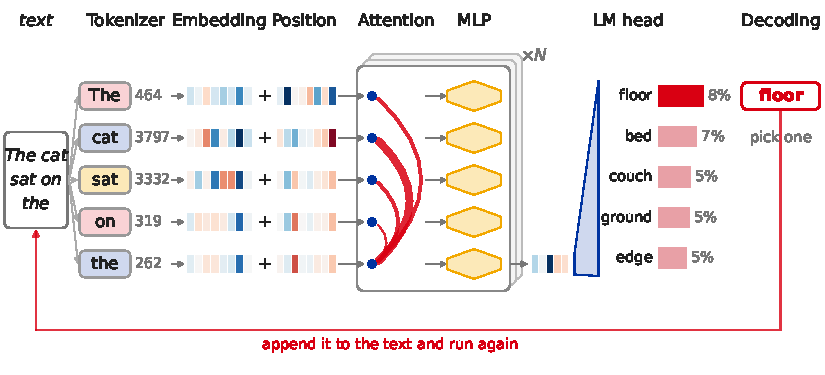
\includegraphics[width=\linewidth]{roadmap_evaluation_pass.pdf}\end{center}
  \vskip -2pt
  {\small The pass writes a fluent answer whether or not it is right. Today: telling which.}
\end{frame}

\begin{frame}{Where we are: the life of a model}
  \begin{center}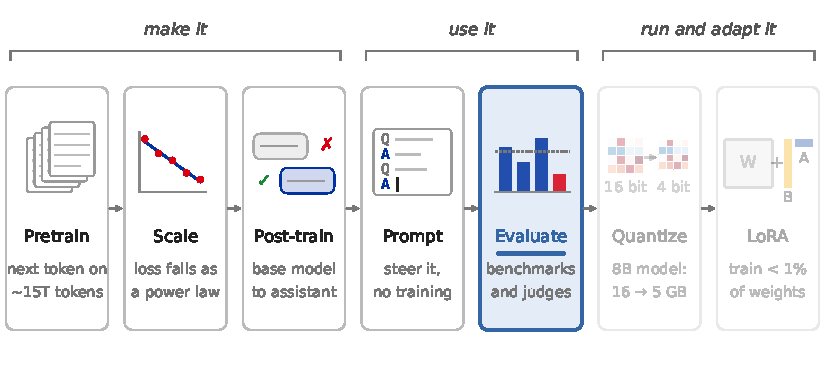
\includegraphics[width=\linewidth]{roadmap_evaluation_life.pdf}\end{center}
  \vskip -2pt
  {\small Today: the last box of ``use it''. Measuring a model, and catching it when it is wrong.}
\end{frame}

% ============================================================ COLD OPEN (py_src/eval_figs.py --gpt2)
\begin{frame}{Ask twice}
  \vskip 6pt
  LLM-4's two prompts, back again. This time GPT-2 \emph{samples} at temperature 1 (LLM-6), 20
  times each:
  \vskip 10pt
  \begin{center}
    ``Lionel Messi plays the sport of \ldots'' \\[4pt]
    ``Henrikh Mkhitaryan plays the sport of \ldots''
  \end{center}
  \vskip 10pt
  {\small (LLM-4: GPT-2 knows the first fact, football at 35\%; it misses the second, hockey first,
  football at 5\%.)}

  \vskip 8pt
  \trapbox{\textbf{Predict first:} can you tell which answer to trust \emph{without} knowing the
  truth, just from the 20 samples?}
\end{frame}

\begin{frame}{Agreement is a signal}
  \begin{center}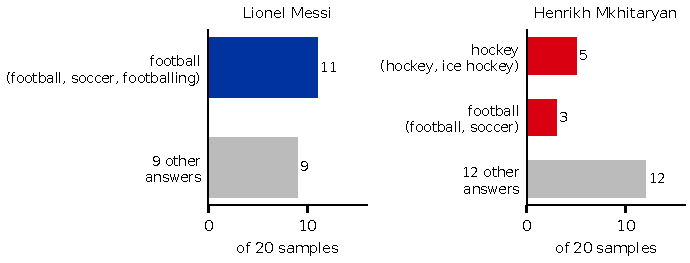
\includegraphics[width=0.72\linewidth]{eval_samples.pdf}\end{center}
  \vskip -4pt
  {\small \textbf{Yes.} Grouped by meaning: Messi's 20 samples use 12 different first words, but 11
  mean football. Mkhitaryan's use 16; the biggest group, hockey (both ``ice'' samples say ``ice
  hockey''), holds 5, and it is wrong. (20 samples are noisy: football 2 in 20 vs 5\% in LLM-4.)}

  \vskip 4pt
  \keybox{A stored fact comes back the same way; a guess scatters. Sample several times and
  measure the agreement, counting answers that \emph{mean} the same as one (two named methods
  at the end).}
\end{frame}

\begin{frame}{Outline}
  \tableofcontents
\end{frame}

% ============================================================ 1. COMPARE WITH A REFERENCE
\section{Compare with a reference}
\sectiontransition{Compare with a reference}{Count the words you share with a known good answer.}

\begin{frame}{Word overlap, by hand}
  \vskip 2pt
  Reference: \texttt{the cat sat on the mat}. What share of a candidate's words (1-grams), and of
  its word pairs (2-grams), appear in the reference? That share is \textbf{n-gram precision}.
  \vskip 6pt
  \begin{center}
  \small
  \begin{tabular}{llcc}
    \toprule
    & \textbf{candidate} & \textbf{words} & \textbf{word pairs} \\
    \midrule
    a right paraphrase & \texttt{a feline rested upon the rug} & 1/6 & 0/5 \\
    close & \texttt{the cat is on the mat} & 5/6 & 3/5 \\
    nonsense & \texttt{the mat sat on the cat} & \textbf{6/6} & \textbf{4/5} \\
    \bottomrule
  \end{tabular}
  \end{center}

  \vskip 6pt
  {\small Each candidate word counts at most as often as it appears in the reference (``the''
  twice). \textbf{BLEU} (translation) is built on this precision: how much of the candidate is in
  the reference. \textbf{ROUGE} (summaries) asks the reverse, recall: how much of the reference
  the candidate covers.}

  \vskip 4pt
  \trapbox{The nonsense sentence gets a perfect word score; the correct paraphrase gets almost
  nothing. Overlap measures wording, not meaning.}
\end{frame}

\begin{frame}{What overlap is for}
  \vskip 6pt
  \begin{itemize}
    \item It works when the answer's \emph{wording} is fairly fixed: translation and
      summarisation against several reference texts, averaged over thousands of sentences. It is
      cheap, fast and repeatable.
    \item It fails for open answers: a good answer to ``explain attention'' can share almost no
      words with any reference.
    \item Comparing embeddings (LLM-2) instead of words catches paraphrases (``feline'' near
      ``cat''), but still cannot tell a fluent wrong answer from a right one.
  \end{itemize}

  \vskip 10pt
  \keybox{For open-ended answers, someone has to read them and judge. At scale, that someone is
  usually another model.}
\end{frame}

% ============================================================ 2. ASK ANOTHER MODEL
\section{Ask another model}
\sectiontransition{Ask another model}{A model reads the answer and grades it.}

\begin{frame}{LLM-as-judge}
  \vskip 6pt
  \begin{itemize}
    \item \textbf{Pointwise}: ``Score this answer from 1 to 10.'' \quad \textbf{Pairwise}:
      ``Which of A and B is better?''
    \item Why use a model at all: no formula decides whether an answer is helpful or correct. A
      person can, but not 10,000 times a night.
    \item Zheng et al. (2023): strong judges (GPT-4) agreed with human preferences over 80\% of the
      time - the same level at which two humans agree with each other.
  \end{itemize}

  \vskip 10pt
  \watchbox{80\% agreement is good, not perfect, and it was measured on one kind of question.
  Check it on yours before you trust it.}
\end{frame}

\begin{frame}{Its biases}
  \vskip 6pt
  Zheng et al. (2023) name three, plus limited reasoning:
  \vskip 4pt
  \begin{itemize}
    \item \textbf{Position}: preferring whichever answer is shown first (or second). Fix: ask
      twice with A and B swapped; count a win only if both orders agree, otherwise a tie.
    \item \textbf{Verbosity}: preferring the longer answer, even when it adds nothing.
    \item \textbf{Self-enhancement}: preferring answers written by the judge's own model family.
  \end{itemize}

  \vskip 10pt
  \trapbox{The same kind of habit as LLM-9's reward hacking: a model optimised against a judge will
  learn the judge's tastes, not just what people wanted.}
\end{frame}

\begin{frame}{How to use a judge without lying to yourself}
  \vskip 4pt
  \begin{itemize}
    \item \textbf{Decompose the task.} ``Is this statement supported, yes or no'' is a question a
      model answers well. ``Score this answer out of 10'' is not.
    \item \textbf{Calibrate once against humans.} Label 50 examples yourself. If the judge agrees
      with you much less often than people agree with each other (about 80\%), its scores are
      decoration.
    \item \textbf{Use it for comparison, never as an absolute.} ``0.81'' means nothing. ``0.81
      versus 0.74 for last week's version, same judge, same questions'' means something.
    \item \textbf{Freeze the judge.} Change the judge model or its prompt and every earlier number
      stops being comparable. Version it like code.
  \end{itemize}

  \vskip 6pt
  \trapbox{Never let the judge be the same model, with the same prompt, as the generator. You are
  asking it to mark its own homework.}
\end{frame}

% ============================================================ 3. USE A TEST SET
\section{Use a test set}
\sectiontransition{Use a test set}{Fixed questions with known answers.}

\begin{frame}{Benchmarks}
  \vskip 6pt
  \begin{itemize}
    \item A benchmark is a fixed set of questions with checkable answers: knowledge (MMLU, LLM-8),
      maths, code with unit tests, multi-step agent tasks.
    \item It is a \emph{sample} of skills. A score says how the model did on those questions, in
      that format, scored that way - nothing more.
    \item Leaderboards turn a score into a target. Goodhart's law (LLM-9): once a measure becomes
      a target, it stops being a good measure - models get tuned to the test.
  \end{itemize}

  \vskip 10pt
  \keybox{A benchmark answers ``better than last month on these questions?'' well, and ``good at
  the job?'' poorly.}
\end{frame}

\begin{frame}{Contamination}
  \begin{columns}[c]
    \column{0.58\textwidth}
      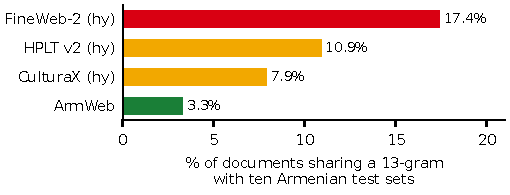
\includegraphics[width=\linewidth]{eval_contamination.pdf}
    \column{0.40\textwidth}
      {\small Four Armenian training corpora, scanned against ten Armenian test sets for 13 words
      in a row copied exactly (a 13-gram). Almost all of the overlap is with the web-derived test
      sets; the hand-built multiple-choice sets: 0.06\% or less in every corpus.}
  \end{columns}

  \vskip 6pt
  {\small \textbf{Contamination}: test questions that are also in the training data. LLM-7's
  lesson: a model holds what it saw, so a contaminated item measures recall, not skill. The same
  study found FineWeb-2's own Armenian \emph{test} split overlapping its \emph{training} split.}
  \vskip 4pt
  \trapbox{Web-scraped test sets end up in web-scraped training sets. Prefer hand-built or newly
  written test questions, and check the overlap before you trust a score.}
  \src{Avetisyan et al. (2026), arXiv 2609.03350 (the arm-gemma-e4b paper).}
\end{frame}

% ============================================================ 4. CONFIDENTLY WRONG
\section{Confidently wrong}
\sectiontransition{Confidently wrong}{Fluent, plausible, and false.}

\begin{frame}{Hallucination}
  \vskip 6pt
  \begin{itemize}
    \item \textbf{Factuality} errors: wrong about the world (``Mkhitaryan plays hockey'' - he is a
      footballer).
    \item \textbf{Faithfulness} errors: wrong about the source you gave it - a summary that adds a
      claim the document never made (the RAG chapter measures this).
    \item Why it happens: the model always produces \emph{some} next token (LLM-5), and a fluent
      wrong one looks exactly like a fluent right one. Nothing in next-token training forces
      ``I don't know''.
  \end{itemize}

  \vskip 10pt
  \keybox{Kalai et al. (2025) add a second reason: our tests reward guessing. Their fix is a
  confidence target $t$: answer only if you are more than $t$ sure.}
\end{frame}

\begin{frame}{Guess or abstain, by hand}
  \begin{columns}[c]
    \column{0.56\textwidth}
      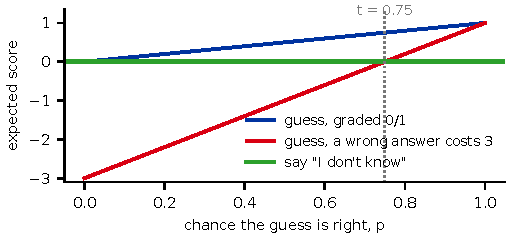
\includegraphics[width=\linewidth]{eval_guess.pdf}
    \column{0.42\textwidth}
      {\small A question the model gets right with probability $p$ if it guesses. ``I don't know''
      scores 0.

      \vskip 4pt
      \textbf{Graded 0/1}: guessing scores $p$ on average, more than 0 for any $p$. Always guess.

      \vskip 4pt
      \textbf{A wrong answer costs 3}: guessing scores $p - 3(1-p)$. At $p = 0.5$: $-1.0$; at
      $p = 0.8$: $+0.2$. Guess only above 0.75.}
  \end{columns}

  \vskip 6pt
  \takebox{Kalai et al.: ``Answer only if you are $> t$ confident, since mistakes are penalized
  $t/(1-t)$ points.'' $t = 0.75$ gives $0.75/0.25 = 3$. Most benchmarks grade 0/1 ($t = 0$),
  which teaches models to guess.}
  \src{Kalai et al. (2025). The paper's own example says ``penalty 2'' for $t = 0.75$; its formula
  gives 3. We use the formula.}
\end{frame}

\begin{frame}{Catching it}
  \vskip 6pt
  \begin{itemize}
    \item \textbf{Ask several times} (the cold open): SelfCheckGPT (Manakul et al., 2023) samples
      the model again and checks each claim of the answer against every sample (with a similarity
      score or another model); claims the samples do not back up are flagged.
    \item \textbf{Count meanings, not words}: semantic entropy (Farquhar et al., 2024) groups the
      samples by meaning first, then measures the spread. Messi: one meaning holds 11 of 20, low
      spread. Mkhitaryan: the biggest holds 5, high spread - distrust it.
    \item \textbf{Ground it}: give the model the documents and check the answer against them. That
      is the next chapter.
  \end{itemize}

  \vskip 10pt
  \watchbox{Agreement catches guesses, not shared mistakes: a model that learned a wrong fact
  well repeats it every time.}
\end{frame}

% ============================================================ CLOSE
\begin{frame}{Recap}
  \small
  \begin{itemize}
    \item \textbf{Reference}: word overlap (BLEU, ROUGE) is cheap and measures wording, not meaning
      - the nonsense sentence scored 6/6.
    \item \textbf{Judge}: over 80\% agreement with people, with position, verbosity and
      self-preference biases; decompose, calibrate, compare, freeze.
    \item \textbf{Test set}: a sample of skills; contamination turns it into a memory test
      (FineWeb-2's Armenian documents: 17.4\%).
    \item \textbf{Hallucination}: no built-in ``I don't know'', and 0/1 grading rewards guessing.
      Sampling agreement is a cheap detector.
  \end{itemize}
\end{frame}

\begin{frame}{Next: the RAG chapter}
  \begin{center}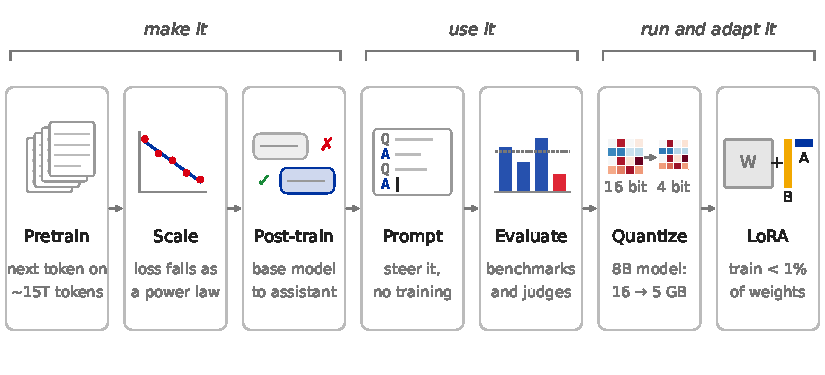
\includegraphics[width=\linewidth]{roadmap_overview_life.pdf}\end{center}
  \vskip -2pt
  {\small Next (L41): give the model the documents - RAG. Then agents (L44), then LLM-12.}
\end{frame}

\begin{frame}{Sources \& further reading}
  \footnotesize
  \begin{itemize}
    \item Papineni et al. (2002), ``BLEU''; Lin (2004), ``ROUGE''.
    \item Zheng et al. (2023), ``Judging LLM-as-a-Judge with MT-Bench and Chatbot Arena''.
    \item Avetisyan et al. (2026), ``From Zero to Hero: An Open LLM Ecosystem for Armenian'', arXiv
      2609.03350 (corpus contamination).
    \item Kalai, Nachum, Vempala \& Zhang (2025), ``Why Language Models Hallucinate''.
    \item Manakul et al. (2023), ``SelfCheckGPT''; Farquhar et al. (2024), ``Detecting
      hallucinations in large language models using semantic entropy'', \emph{Nature}.
  \end{itemize}
  \vskip 2pt
  \src{Figures: \texttt{py\_src/eval\_figs.py}. Real: GPT-2's 20 samples per prompt (cached model,
  seed 509) and the published contamination rates. Toy: the overlap table and the guessing
  plot.}
\end{frame}

\end{document}

% ============================================================================
% Provenance:
%   Deck: LLM-11 Evaluation and hallucination (14_llms), session 11. Built 2026-10-06 from
%   LLM11_evaluation_OUTLINE.md, which follows the critique in LLM_CHAPTER_PLAN.md (LLM-11) and the
%   recommended answers in INTERVIEW_QUEUE.md (instructor: "do all queue items"): the four-ways
%   spine; the sampling demo on LLM-4's prompts (cached GPT-2, T = 1, 20 samples, seed 509);
%   published judge findings only (no paid API); Kalai et al.'s guess-vs-abstain table.
%   RAG item 3 (judges): "How to use a judge without lying to yourself" moved here from L43, which
%   keeps its two RAG-specific judge frames and now points back (same day).
%   Sources ported: dl4nlp 05 (BLEU/ROUGE, judges, benchmarks, contamination; perplexity -> LLM-7,
%   MAP/nDCG -> L43) and 09 (taxonomy, SelfCheckGPT, semantic entropy; RAG mitigation -> ch17).
%   Facts checked 2026-10-06 (outline table): Zheng and Kalai abstracts, Kalai's confidence-target
%   text (whose "t = 0.75 (penalty 2)" disagrees with its own t/(1-t) - the slide says so), the
%   Armenian contamination numbers in arXiv 2609.03350's full text.
%   Every printed number is asserted in py_src/eval_figs.py (the overlap fractions, the sample
%   counts by word and by meaning, the entropies, the expected scores, t = 0.75 -> 3).
%   "Next": the overview map (the RAG chapter is not on the LLM map) with the teaching order.
%   STUDENT REVIEW 2026-10-06 (one Sonnet agent, rendered PNGs only; ~77k tokens, 63 s). It re-did
%   the overlap fractions, the sample totals and the expected scores and found none wrong.
%   Applied: the samples chart grouped by meaning (the 11 and the 5 readable; "ice" = "ice hockey",
%   checked); the predict-first answered ("Yes"); the noise caveat (2 in 20 vs 5%); n-gram
%   precision, BLEU precision vs ROUGE recall, contamination and 13-gram defined; the judge
%   calibration tied to the 80% human level; the tie rule; Goodhart restated; which test sets
%   carry the overlap; t introduced before the plot; the penalty footnote made plain;
%   SelfCheckGPT's check and a semantic-entropy reading of the cold open.
% ============================================================================
